\documentclass{beamer}

\usepackage{graphicx}
\usepackage{amsmath}
\usepackage{hyperref}
\usepackage{tikz}
\usepackage{booktabs} 

% Title page
\title{What are the Most Important Statistical Ideas of the Past 50 Years?\\
\vspace{0.5em}
\small Andrew Gelman and Aki Vehtari}
\author{Faryal Fodderwala}
\date{\today}

\begin{document}

% Title Slide
\frame{\titlepage}

% Slide 1: Introduction
\begin{frame}{Introduction}
\begin{itemize}
    \item Overview of 8 significant statistical ideas from 1970 to 2021.
    \item Authors: Andrew Gelman and Aki Vehtari.
    \item Purpose: To provoke thought and discussion about modern statistical innovations and their impact on data science.
\end{itemize}
\end{frame}

% Slide 2: Authors' Background
\begin{frame}{Authors' Background}
\begin{minipage}{0.3\textwidth}
    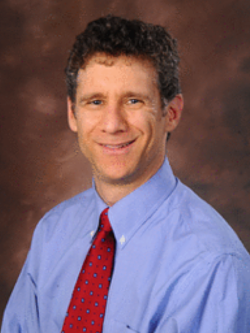
\includegraphics[width=\textwidth]{andrew_gelman.png} 
    \centering
    \small Andrew Gelman
\end{minipage}
\hfill
\begin{minipage}{0.65\textwidth}
    \begin{itemize}
        \item \textbf{Andrew Gelman}:
        \begin{itemize}
            \item Professor of Statistics and Political Science, Columbia University.
            \item Renowned for Bayesian statistics and multilevel modeling.
        \end{itemize}
    \end{itemize}
\end{minipage}

\vspace{1em}

\begin{minipage}{0.3\textwidth}
    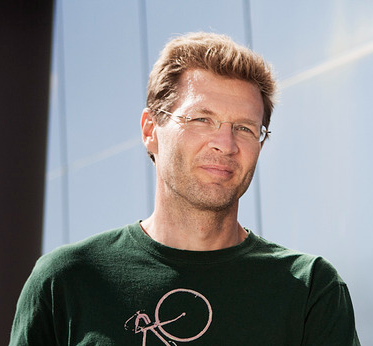
\includegraphics[width=\textwidth]{aki_vehtari.png} 
    \small Aki Vehtari
\end{minipage}
\hfill
\begin{minipage}{0.65\textwidth}
    \begin{itemize}
        \item \textbf{Aki Vehtari}:
        \begin{itemize}
            \item Professor of Computational Probabilistic Modeling, Aalto University.
            \item Focused on Bayesian computation and model assessment.
        \end{itemize}
    \end{itemize}
\end{minipage}
\end{frame}

% Slide: Bayesian Data Analysis and the Authors' Authority
\begin{frame}{Authors' Background (cont.)}
\vspace{0.5em} 
\begin{minipage}{0.35\textwidth}
    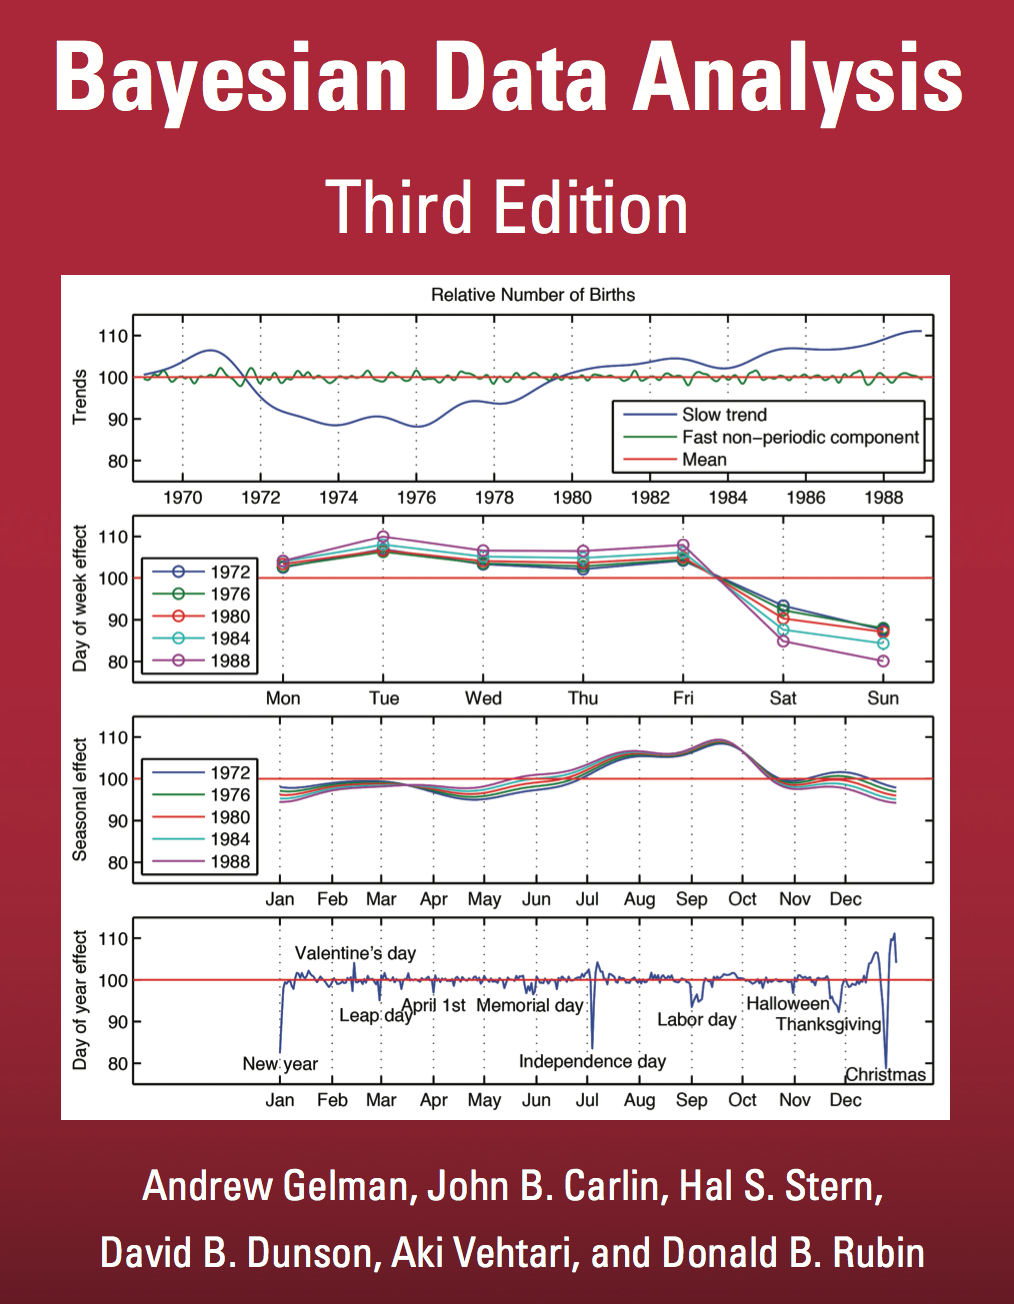
\includegraphics[width=\textwidth]{bayesian_data_analysis_cover.png}
    \centering
    \small \textit{Bayesian Data Analysis}
\end{minipage}
\hfill
\begin{minipage}{0.6\textwidth}
    \small 
    \begin{itemize}
        \item \textbf{The Book: Bayesian Data Analysis}
        \begin{itemize}
            \item Written by Andrew Gelman, Aki Vehtari, and others.
            \item Widely regarded as the foundational text ("the bible") for Bayesian practitioners.
            \item Covers theory, computation, and applied Bayesian methods.
        \end{itemize}
        \vspace{0.5em} 
        \item \textbf{Their Authority on the Topic}
        \begin{itemize}
            \item Through this book, Gelman and Vehtari have shaped the modern understanding of Bayesian statistics.
            \item Their extensive research and contributions give them unique insights to answer: \textit{What are the most important statistical ideas of the past 50 years?}
        \end{itemize}
    \end{itemize}
\end{minipage}
\end{frame}



% Slide: Statistical Modeling Blog
\begin{frame}{Gelman's Blog}
\begin{center}
    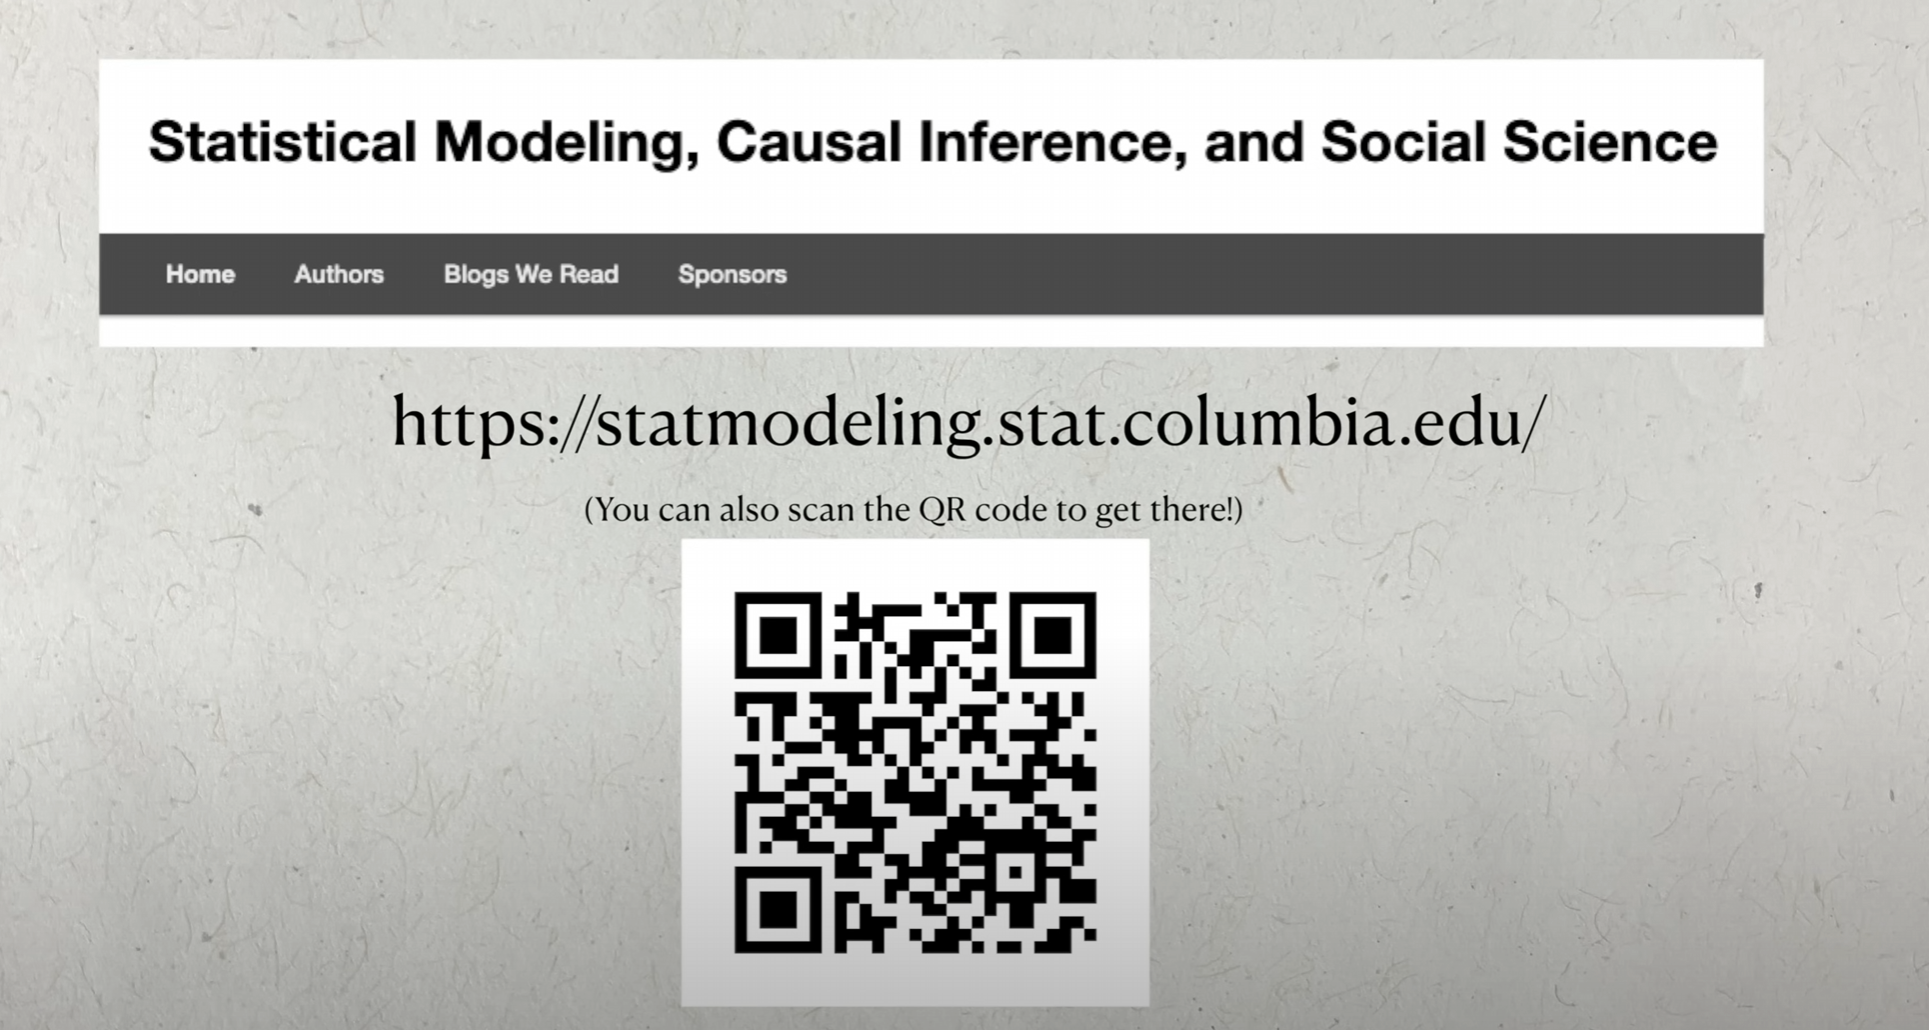
\includegraphics[width=\textwidth]{statistical_modeling_blog.png}
\end{center}
\end{frame}


% Slide 3: Overview of the Paper
\begin{frame}{Overview of the Paper}
\begin{itemize}
    \item Timeframe: 1970 to 2021, focusing on the development of modern statistics.
    \item 8 statistical ideas selected based on their influence on statistical theory, computation, and applications.
    \item Published to the \textit{Journal of the American Statistical Association} as an \textbf{essay}, not a research manuscript.
            \item Acknowledges that no definitive list can encompass all significant ideas.
\end{itemize}
\end{frame}

% Slide: Key Statistical Concepts
\begin{frame}{Key Statistical Concepts}
\textbf{The 8 Statistical Ideas Covered in the Paper:}
\begin{enumerate}
    \item Counterfactual Causal Inference
    \item Bootstrapping and Simulation-Based Inference
    \item Overparameterized Models and Regularization
    \item Bayesian Multilevel Models
    \item Generic Computation Algorithms
    \item Adaptive Decision Analysis
    \item Robust Inference
    \item Exploratory Data Analysis (EDA)
\end{enumerate}

\vspace{0.5cm}

\textbf{Purpose:} These concepts reflect significant innovations in statistical theory, computation, and application from the last 50 years.
\end{frame}


% Slide: Intro to Counterfactual Causal Interference
\begin{frame}{The Challenge of Observational Data}
\begin{itemize}
    \item \textbf{In an ideal world: Experimental Data}
    \begin{itemize}
        \item Researchers control interventions.
        \item Participants are assigned to "treatment" and "control" groups.
        \item Enables \textit{causal claims} about the effect of an intervention.
    \end{itemize}
    \item \textbf{In the real world: Observational Data}
    \begin{itemize}
        \item Researchers cannot control who receives the intervention.
        \item Only allows for \textit{correlational claims}.
        \item Several fields of study are prone to having more observational data i.e. statistics, econometrics, psychometrics, epidemiology, and computer science.
    \end{itemize}
\end{itemize}

\vspace{0.5cm}

\textbf{Challenge:} How can we infer causality in the absence of experimental data?
\end{frame}

% Slide: Introducing Counterfactuals
\begin{frame}{Introducing Counterfactuals}
\begin{itemize}
    \item \textbf{Model Setup:}
    \begin{itemize}
        \item Let \(X\) represent attending class:
        \begin{itemize}
            \item \(x = 0\): Did not attend class.
            \item \(x = 1\): Did attend class.
        \end{itemize}
        \item In reality, I choose to attend class and receive a score \(Y_1\) on my paper.
    \end{itemize}
    
    \vspace{0.3cm}
    
    \item \textbf{Key Question:} Did attending class improve my score?
    \begin{itemize}
        \item To answer this, we need to consider an alternative reality:
        \item What score (\(Y_0\)) would I have received if I \textit{did not} attend class?
    \end{itemize}
\end{itemize}

\vspace{0.5cm}

\textbf{Key Idea: Counterfactuals}
\begin{itemize}
    \item \(Y_0\): The score in the unobserved reality (if I did not attend class).
    \item This unobserved reality is called the \textit{counterfactual}.
\end{itemize}
\end{frame}


% Slide 4: Counterfactual Causal Inference
\begin{frame}{01: Counterfactual Causal Inference}
\begin{itemize}
    \item Allows causal inference using observational data.
    \item Framework based on "potential outcomes" or "counterfactuals."
\end{itemize}

\[
\text{Causal Effect: } Y(1) - Y(0)
\]
\begin{itemize}
    \item \( Y(1) \): Outcome if treated.
    \item \( Y(0) \): Outcome if untreated.
    \item Challenge: Only one outcome is observed.
\end{itemize}
\end{frame}

% Slide 5: Bootstrapping and Simulation-Based Inference
\begin{frame}{02: Bootstrapping and Simulation-Based Inference}
\begin{itemize}
    \item Introduced by Bradley Efron (1979).
    \item Resampling technique to estimate sampling distributions without assumptions about data distribution.
\end{itemize}

\begin{exampleblock}{Algorithm:}
\begin{enumerate}
    \item Resample the dataset with replacement.
    \item Compute the statistic of interest (e.g., mean).
    \item Repeat \( n \) times to estimate variability.
\end{enumerate}
\end{exampleblock}
\end{frame}

% Slide: Bootstrapping and Simulation-Based Inference (cont.)
\begin{frame}{02: Bootstrapping and Simulation-Based Inference (cont.)}
\begin{itemize}
    \item \textbf{The Bootstrap Algorithm:}
    \begin{center}
        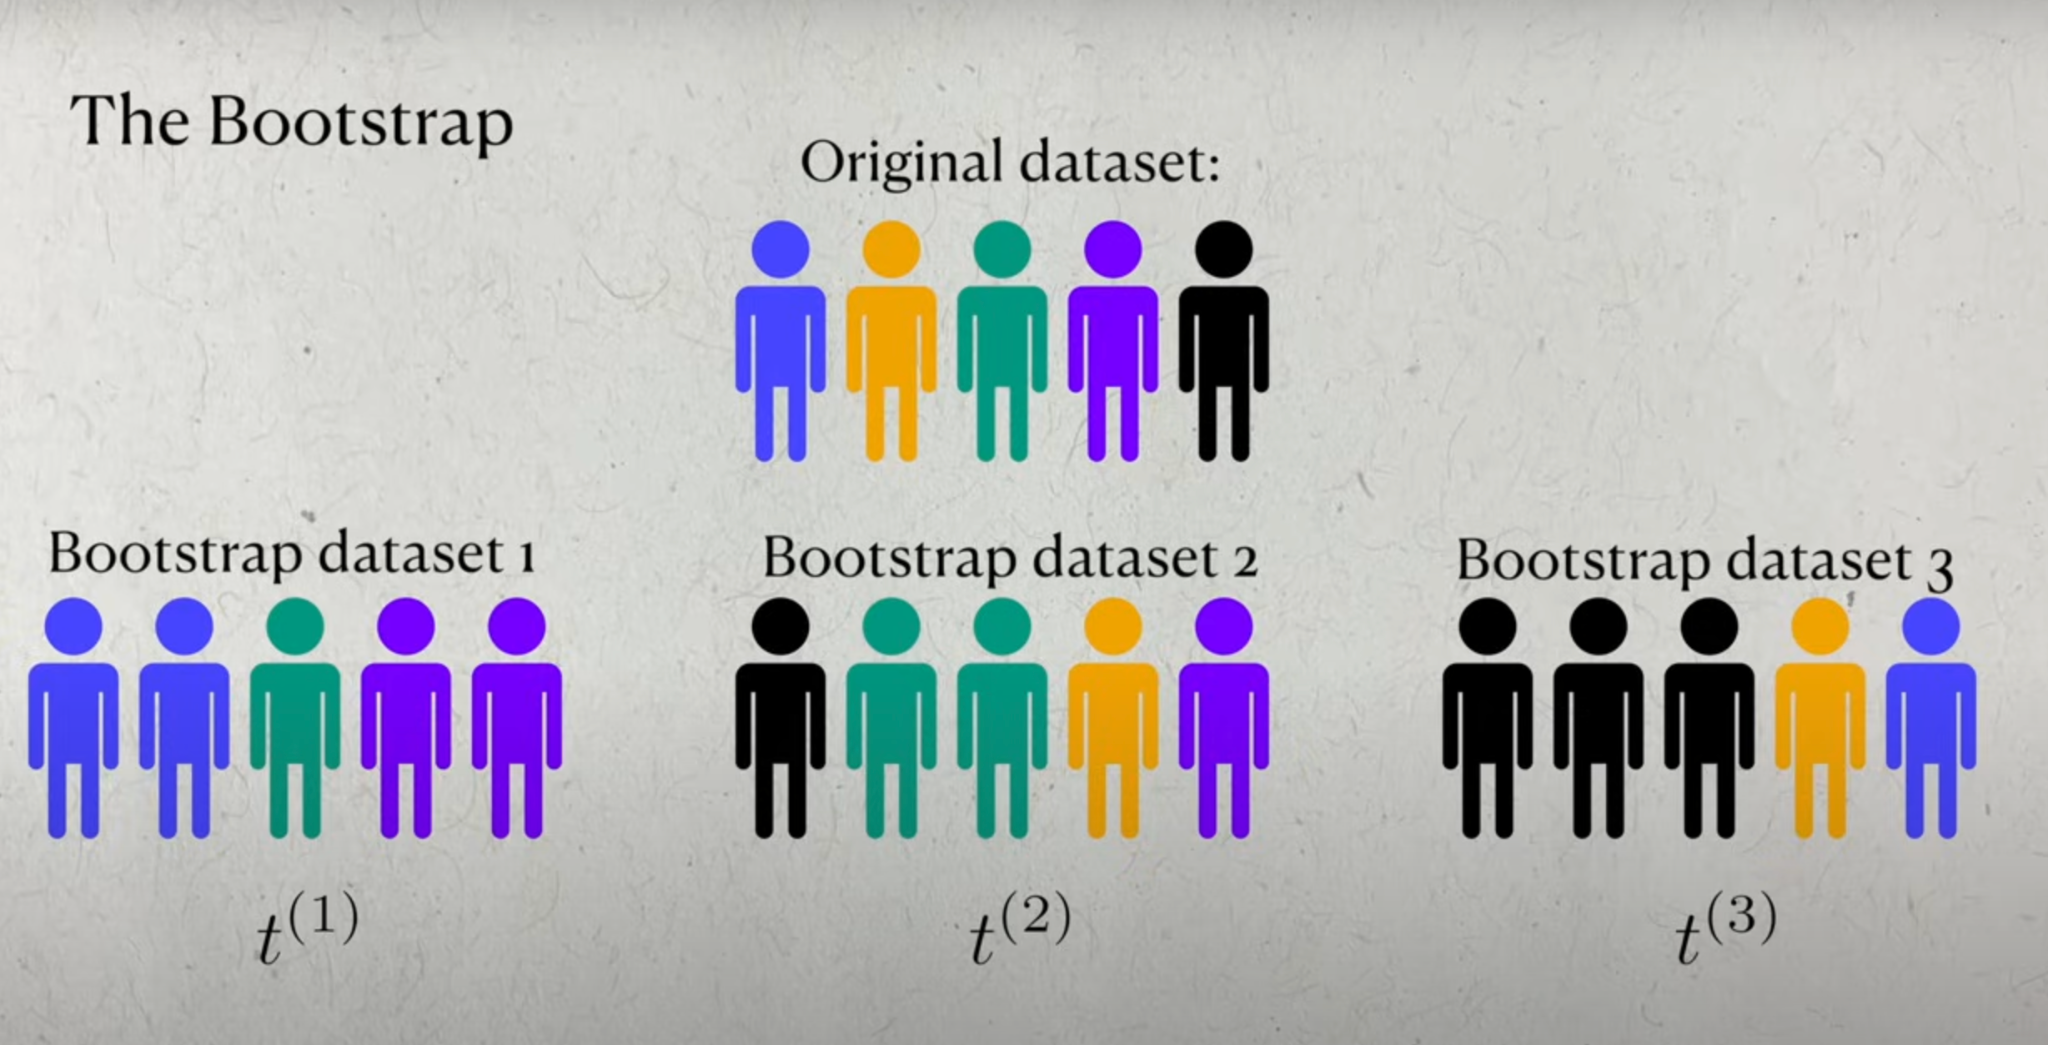
\includegraphics[width=0.7\textwidth]{bootstrap_populations.png}
    \end{center}
    \item \( \hat{F}(t) \) Goal: Estimate the CDF of some statistic.
    \item \textbf{Intuition:} Data sampled from the original dataset resembles a new dataset.
    \item For each bootstrap dataset, calculate a statistic of interest and derive its distribution:
    \[
    t^{(1)}, t^{(2)}, t^{(3)} \to \hat{F}(t)
    \]
\end{itemize}
\end{frame}


% Slide: Simulation-Based Inference
\begin{frame}{Simulation-Based Inference (cont.)}
\begin{itemize}
    \item \textbf{Example using Bayes' Rule:}
    \[
    P(\theta \mid X) = \frac{P(X \mid \theta) \colorbox{blue!20}{$P(\theta)$}}{P(X)}
    \]

    \item \textbf{Bayesian Approach:}
    \begin{itemize}
        \item Bayesian encodes knowledge in the form of prior distributions.
        \item Conduct \textbf{prior predictive checks:}
        \[
        P(\Theta) \to \Theta \to X
        \]
        Checks if the data generated from the prior distribution aligns with realistic or expected values.
        \item Conduct \textbf{posterior predictive checks:}
        \[
        P(\Theta \mid X) \to \Theta \to X^*
        \]
        Evaluates how well the posterior distribution predicts new or observed data points.
    \end{itemize}

    \item \textbf{Rise of Computational Power:}
    \begin{itemize}
        \item Advances in computational power have made simulations easier and more widely applicable.
    \end{itemize}
\end{itemize}
\end{frame}




% Slide: Overparameterized Models and Regularization
\begin{frame}{03: Overparameterized Models and Regularization}
\begin{itemize}
    \item Adding parameters to a model allows for more flexibility and complexity:
    
    \textbf{Model 1: Simple Linear Regression} \\
    \[
    Y_i = \beta_0 + \beta_1 X_i + \epsilon_i
    \]
    \vspace{-1em}
    \begin{itemize}
        \item Explains the relationship between an outcome (\(Y\)) and a predictor (\(X\)).
        \item Limitation: Cannot account for time-varying effects or individual differences.
    \end{itemize}

    \textbf{Model 2: Incorporating More Parameters} \\
    \[
    Y_i = \beta_0 + \beta_1 X_i + \beta_2 \text{time} + \beta_3 (X_i \cdot \text{time}) + \epsilon_i
    \]
    \vspace{-1em}
    \begin{itemize}
        \item Adds parameters for time and its interaction with treatment, increasing flexibility.
        \item Still assumes uniform responses across individuals.
    \end{itemize}
\end{itemize}
\end{frame}

% Slide: Overparameterized Models and Regularization (cont.)
\begin{frame}{03: Overparameterized Models and Regularization (cont.)}
\scriptsize
\textbf{Model 3: Mixed Effects Model (More Parameters, More Flexibility)}
\[
Y_i = \beta_0 + b_{0i} + \beta_1 X_i + b_{1i} X_i + \beta_2 \text{time} + \beta_3 (X_i \cdot \text{time}) + \epsilon_i
\]
\vspace{-1em}
\begin{itemize}
    \item Includes subject-specific random effects (\(b_{0i}, b_{1i}\)), allowing for individual-level flexibility, increases model complexity.
\end{itemize}


\textbf{Example: Neural Networks}
\begin{itemize}
    \item Overparameterized models take these models to the extreme, with hundreds or thousands of parameters.
    \item In neural networks, each edge in the network is associated with a parameter or weight. By making these networks very large, they can approximate a wide variety of functions (\textbf{Universal Approximation Theorem}).
\end{itemize}

\begin{center}
    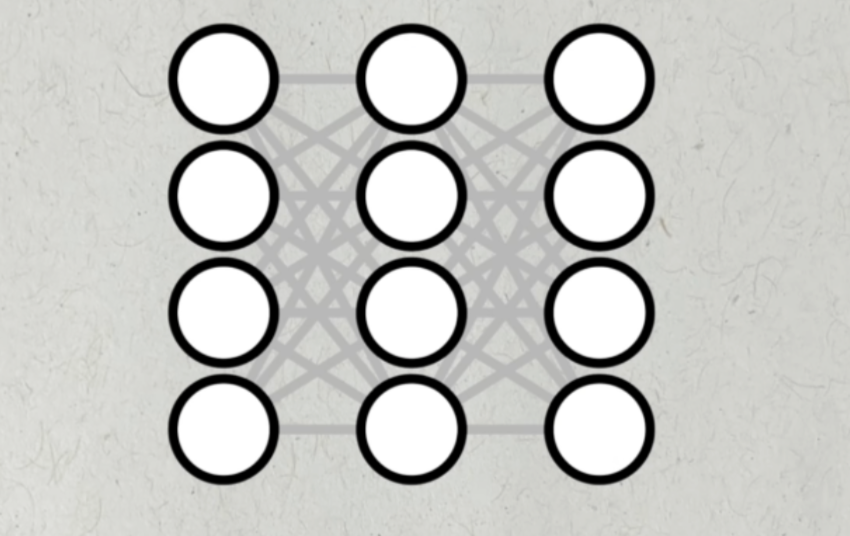
\includegraphics[width=0.5\textwidth]{neural_network.png}
\end{center}

\end{frame}



% Slide 7: Multilevel Models (Part 1)
\begin{frame}{04: Bayesian Multilevel Models}
\begin{itemize}
    \item Multilevel (or hierarchical) models assume a structure over parameters.
    \item These models allow for varying effects at different levels of hierarchy:
    \begin{itemize}
        \item \textbf{First-level units:} Generate treatment effects.
        \item \textbf{Second-level units:} Generate observed data and can vary depending on the research question.
    \end{itemize}
    \item Example: Aggregating data across different groups in meta-analysis.
\end{itemize}

\begin{center}
    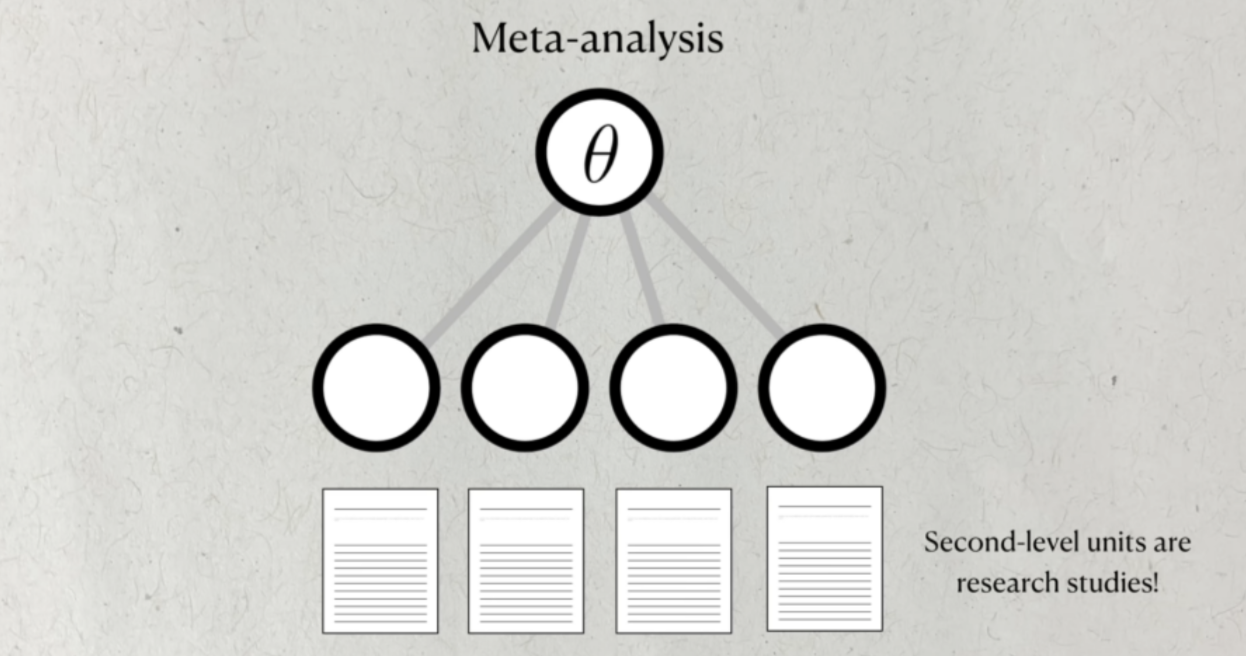
\includegraphics[width=0.8\textwidth]{meta_analysis.png}
\end{center}
\end{frame}

% Slide 8: Multilevel Models (Part 2)
\begin{frame}{04: Bayesian Multilevel Models (cont.)}
\begin{itemize}
    \item The structure of the multilevel model can be expressed as:
    \[
    y_{ij} = \beta_0 + \beta_1 X_{ij} + u_j + \epsilon_{ij}
    \]
    \item Definitions:
    \begin{itemize}
        \item \( u_j \): Random effect for group \( j \).
        \item \( \epsilon_{ij} \): Error term for observation \( i \) in group \( j \).
    \end{itemize}
\end{itemize}

\begin{block}{Advantage}
\begin{itemize}
\item Combines individual-level and group-level variability for improved estimates.
\item The Bayesian framework offers more flexibility in the modeling approach, as the choice of prior distributions plays a major role in capturing uncertainties and incorporating domain knowledge.
\end{itemize}
\end{block}
\end{frame}



% Slide 1: Generic Computation Algorithms
\begin{frame}{05: Generic Computation Algorithms}
\begin{itemize}
    \item \textbf{Importance of Computers in Statistics:}
    \begin{itemize}
        \item Advances in computational power have been crucial for enabling and implementing complex statistical models.
        \item Algorithms like EM and Metropolis-Hastings make it possible to analyze data that would otherwise be computationally infeasible.
    \end{itemize}
\end{itemize}
\end{frame}

% Slide 2: The Expectation-Maximization (EM) Model
\begin{frame}{The Expectation-Maximization (EM) Model}
\begin{itemize}
    \item \textbf{Purpose:} Solves estimation problems when data is incomplete or latent.
    \item \textbf{Process:} Uses available data to construct educated guesses for parameter values in a model (\(\hat{\theta} \to \theta\)).
    \item \textbf{Example:} Mixture models with latent classes, where group labels are unknown. The EM algorithm estimates parameters even without direct class information.
\end{itemize}
\end{frame}

% Slide 3: Metropolis-Hastings (M-H)
\begin{frame}{Metropolis-Hastings (M-H)}
\begin{itemize}
    \item \textbf{Purpose:} Allows sampling from complex distributions that are difficult to handle mathematically.
    \item \textbf{Bayesian Context:}
    \begin{itemize}
        \item In Bayes' rule, the posterior distribution \( P(\theta \mid X) \) can be so complicated that we cannot derive a closed-form formula for it.
        \item M-H generates data samples directly from this posterior, enabling us to:
        \begin{itemize}
            \item Recover key quantities like means, quantiles, and credible intervals.
        \end{itemize}
    \end{itemize}
    \item \textbf{Importance:} Demonstrates the power of computation in Bayesian statistics, as it bypasses analytical challenges.
\end{itemize}
\end{frame}


% Slide 9: Adaptive Decision Analysis
\begin{frame}{06: Adaptive Decision Analysis}
\begin{itemize}
    \item \textbf{Framework for Decision-Making:}
    \begin{itemize}
        \item Interim decision points: Collect and analyze data before the experiment concludes.
    \end{itemize}
    \item \textbf{Application:} Stopping clinical stem cell trials early:
    \begin{itemize}
        \item If evidence suggests treatment is futile, the trial can be stopped early.
        \item If treatment shows early promise, the trial may also be stopped to proceed with broader application.
        \item A well-designed trial allows us to control the consequences of our decision, such as type I error.
    \end{itemize}
    \item \textbf{Frequentist Considerations:}
    \begin{itemize}
        \item Stopping early may hurt power and complicate the interpretation of the \( p \)-value.
    \end{itemize}
\end{itemize}
\end{frame}


% Slide 10: Robust Inference
\begin{frame}{07: Robust Inference}
\begin{itemize}
    \item Statisticians often make assumptions about their models. When assumptions are reasonable, results can generally be presumed trustworthy.
    \item \textbf{However, assumptions are not always right.}
    \item \textbf{Definition:} Robust statistics provide trustworthy analyses even when some assumptions are incorrect.
\end{itemize}

\begin{block}{Example: Outliers}
\begin{itemize}
    \item Outliers violate assumptions about the distribution of data (e.g., normality).
    \item Median-based estimators are less sensitive to outliers compared to mean-based estimators.
\end{itemize}
\end{block}

\begin{block}{Key Insight}
Robust inference allows valid results even when data deviates from assumptions.
\end{block}
\end{frame}

% Slide 11: Propensity Score Matching
\begin{frame}{Propensity Score Matching}
\begin{itemize}
    \item \textbf{Definition:} A method to match people in a treatment group to people in a control group who are very similar to them.
    \item Propensity Score Matching requires two models:
    \begin{itemize}
        \item \textbf{Model 1: Exposure-Outcome Model}
        \[
        Y_i = \beta_0 + \beta_1 T_i + E_i
        \]
        Estimates the effect of the treatment (\(T_i\)) on the outcome (\(Y_i\)).
        \item \textbf{Model 2: Propensity Score Model}
        \[
        E_i = \tau_0 + \tau_1 C_i
        \]
        Matches individuals based on their covariates (\(C_i\)).
    \end{itemize}
    \item Both models must ideally be correctly specified; however:
    \begin{itemize}
        \item Correct specification is rarely achieved in practice.
        \item Robust versions of Propensity Score Matching allow one model to be misspecified.
    \end{itemize}
    \item \textbf{Key Point:} The fewer assumptions we make, the better. Robust methods provide more reliable causal effect estimates.
\end{itemize}
\end{frame}


% Slide 11: Exploratory Data Analysis (EDA)
\begin{frame}{08: Exploratory Data Analysis (EDA)}
\begin{itemize}
    \item Emphasizes visualization and insights over intense theory and computation.
    \item Useful in understanding the relation between data, fitted model, and predictions.
\end{itemize}

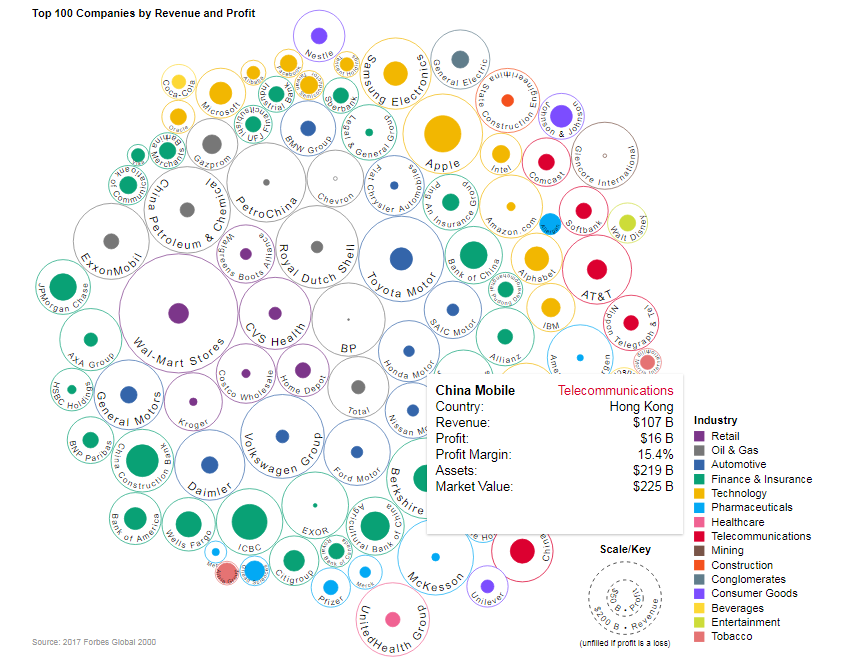
\includegraphics[width=0.9\textwidth]{bubble-chart.png}
\end{frame}

% Slide 12: Connection to NYC Open Data
\begin{frame}{Connection to NYC Open Data}
\begin{itemize}
    \item Apply statistical methods to NYC datasets.
    \item Example: Visualize and analyze restaurant complaints using robust inference and EDA.
\end{itemize}

\begin{center}
  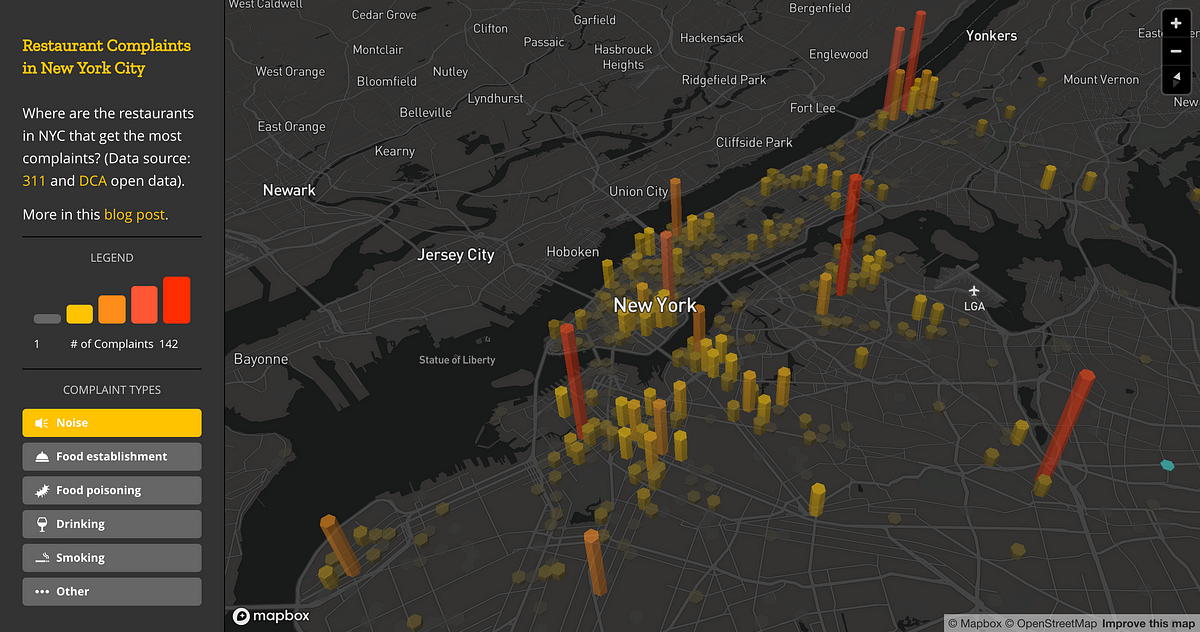
\includegraphics[width=0.9\textwidth]{nyc-open-data.png}
\end{center}

\begin{center}
    \small \url{https://labs.mapbox.com/bites/00304/}
\end{center}
\end{frame}

% Slide: What does it mean for an idea to be important?
\begin{frame}{What does it mean for an idea to be important?}
\begin{itemize}
    \item Gelman emphasized avoiding citation counts of papers where concepts originated.
    \item Instead, he assessed principles that influenced the development of ideas in modern statistical practice.
    \item Example from the literature: The paper "The Importance of Being Clustered" (Anderluci et al., 2019) analyzed trends in statistics from 1970–2015 using clustering techniques to identify influential statistical ideas and themes.
\item \textcolor{red}{\textbf{My Remarks:}}
    \begin{itemize}
        \item \textcolor{red}{Many of these ideas seem to have arisen from the analysis of very large datasets and the challenges inherent in combining sets of data.}
        \item \textcolor{red}{The availability of computational power has also increased the tendency to model these statistical problems, pushing forward the development of modern methods.}
    \end{itemize}
\end{itemize}
\end{frame}




% Slide 14: The Importance of Human Oversight in Statistical Innovations
\begin{frame}{The Importance of Human Oversight in Statistical Innovations}
\begin{itemize}
    \item As computational power advances, machine learning and statistical algorithms can model complex systems.
    \item However, these models are only as good as the assumptions and data they are based on.
    \item Example: Self-driving cars can use machine learning to navigate, but human oversight is needed to determine:
    \begin{itemize}
        \item Are the outcomes (e.g., accident rates) statistically significant?
        \item Are the algorithms operating ethically and equitably?
    \end{itemize}
    \item \textbf{Key Point}: Computational tools are powerful, but without human observation and ethical guidance, they can lead to unintended consequences.
\end{itemize}

\begin{block}{Reflection from Gelman}
\textit{"On one hand, you have all these amazing things that machine learning can do, like self-driving cars, but you'll need a statistician to tell you if the number of people being killed by the self-driving cars is statistically significant."} – Paraphrased from Andrew Gelman in a separate interview
\end{block}

\begin{block}{Looking Ahead}
\begin{itemize}
    \item The 21st century demands statisticians not only develop and deploy algorithms but also critically observe and safeguard their societal impacts.
    \item Ethical and interpretative roles remain as crucial as computational capabilities.
\end{itemize}
\end{block}
\end{frame}



% Slide 14: Questions
\begin{frame}{Questions?}
\begin{center}
    Thank you! Any questions?
\end{center}
\end{frame}

% Slide 15: References
\begin{frame}{References}
\tiny
\begin{itemize}
    \item Gelman, Andrew, and Aki Vehtari. 2021. "What are the Most Important Statistical Ideas of the Past 50 Years?" 
    \textit{Journal of the American Statistical Association}, 116(536): 2087–2097.
    \item Gelman, Andrew. \textit{Statistical Modeling, Causal Inference, and Social Science}. Accessed at: \url{https://statmodeling.stat.columbia.edu/}
    \item Gelman, Andrew. \textit{What are the most important statistical ideas of the past 50 years?} YouTube video. Available at: \url{https://www.youtube.com/watch?v=M6ha2UeSZbo}
    \item Gelman, Andrew. Additional commentary on statistical ideas. YouTube video. Available at: \url{https://youtu.be/nCyGhqQWj2g?si=GM9KpuWtg4tGV8je}
    \item Mapbox. 2018. "Exploring NYC Open Data with 3D Hexbins." Available at: \url{https://blog.mapbox.com/exploring-nyc-open-data-with-3d-hexbins-5af2b7d8bc46}
\end{itemize}

\footnotesize
Images:
\begin{itemize}
    \item bootstrap\_populations.png
    \item neural\_networks.png
    \item meta\_analysis.png
    \item propensity\_score\_matching.png
    \item bubble-chart.png
\end{itemize}
\end{frame}



\end{document}
